\let\negmedspace\undefined
\let\negthickspace\undefined
\documentclass[journal,12pt,onecolumn]{IEEEtran}
\usepackage{cite}
\usepackage{amsmath,amssymb,amsfonts,amsthm}
\usepackage{algorithmic}
\usepackage{graphicx}
\graphicspath{{./figs/}}
\usepackage{textcomp}
\usepackage{xcolor}
\usepackage{txfonts}
\usepackage{listings}
\usepackage{enumitem}
\usepackage{mathtools}
\usepackage{gensymb}
\usepackage{comment}
\usepackage{caption}
\usepackage[breaklinks=true]{hyperref}
\usepackage{tkz-euclide} 
\usepackage{listings}
\usepackage{gvv}    
\usepackage{multicol}




\begin{document}
\title{
ASSIGNMENT 4: GATE 2020\\
GG : Geology and Geophysics}
\author{EE25BTECH11003 -Adharvan Kshathriya Bommagani}
\maketitle
\section*{GA - General Aptitude}

\begin{enumerate}


\item The untimely loss of life is a cause of serious global concern as thousands of people get killed \rule{1cm}{0.15mm} accidents every year while many other die \rule{1cm}{0.15mm} diseases like cardio vascular disease, cancer, etc.

\hfill{\brak{\text{GATE GG 2020}}}
\begin{multicols}{4}
\begin{enumerate}
    \item in, of
    \item from, of
    \item during, from
    \item from, from
\end{enumerate}
\end{multicols}

\item He was not only accused of theft \rule{1cm}{0.15mm} of conspiracy.

\hfill{\brak{\text{GATE GG 2020}}}
\begin{multicols}{4}
\begin{enumerate}
    \item rather
    \item but also
    \item but even
    \item rather than
\end{enumerate}
\end{multicols}

\item Select the word that fits the analogy: \\
Explicit: Implicit :: Express: \rule{1cm}{0.15mm}

\hfill{\brak{\text{GATE GG 2020}}}
\begin{multicols}{4}
\begin{enumerate}
    \item Impress
    \item Repress
    \item Compress
    \item Suppress
\end{enumerate}
\end{multicols}

\item The Canadian constitution requires that equal importance be given to English and French. Last year, Air Canada lost a lawsuit, and had to pay a six-figure fine to a French-speaking couple after they filed complaints about formal in-flight announcements in English lasting 15 seconds, as opposed to informal 5 second messages in French. \\
The French-speaking couple were upset at

\hfill{\brak{\text{GATE GG 2020}}}
\begin{enumerate}
    \item the in-flight announcements being made in English.
    \item the English announcements being clearer than the French ones.
    \item the English announcements being longer than the French ones.
    \item equal importance being given to English and French.
\end{enumerate}

\item A superadditive function $f(\cdot)$ satisfies the following property
$$f(x_{1}+x_{2})\ge f(x_{1})+f(x_{2})$$
Which of the following functions is a superadditive function for $x>1$?

\hfill{\brak{\text{GATE GG 2020}}}
\begin{multicols}{4}
\begin{enumerate}
    \item $e^{x}$
    \item $\sqrt{x}$
    \item $\frac{1}{x}$
    \item $e^{-x}$
\end{enumerate}
\end{multicols}





\item The global financial crisis in 2008 is considered to be the most serious world-wide financial crisis, which started with the sub-prime lending crisis in USA in 2007. The sub-prime lending crisis led to the banking crisis in 2008 with the collapse of Lehman Brothers in 2008. The sub-prime lending refers to the provision of loans to those borrowers who may have difficulties in repaying loans, and it arises because of excess liquidity following the East Asian crisis. \\
Which one of the following sequences shows the correct precedence as per the given passage?

\hfill{\brak{\text{GATE GG 2020}}}
\begin{enumerate}
    \item East Asian crisis $\rightarrow$ subprime lending crisis $\rightarrow$ banking crisis $\rightarrow$ global financial crisis.
    \item Subprime lending crisis $\rightarrow$ global financial crisis $\rightarrow$ banking crisis $\rightarrow$ East Asian crisis.
    \item Banking crisis $\rightarrow$ subprime lending crisis $\rightarrow$ global financial crisis $\rightarrow$ East Asian crisis.
    \item Global financial crisis $\rightarrow$ East Asian crisis $\rightarrow$ banking crisis $\rightarrow$ subprime lending crisis.
\end{enumerate}

\item It is quarter past three in your watch. The angle between the hour hand and the minute hand is

\hfill{\brak{\text{GATE GG 2020}}}
\begin{multicols}{4}
\begin{enumerate}
    \item $0^{\degree}$
    \item $7.5^{\degree}$
    \item $15^{\degree}$
    \item $22.5^{\degree}$
\end{enumerate}
\end{multicols}

\item A degreele with centre O is shown in the figure. A rectangle PQRS of maximum possible area is inscribed in the degreele. If the radius of the degreele is a, then the area of the shaded portion is

\hfill{\brak{\text{GATE GG 2020}}}
\begin{figure}[h!]
    \centering
    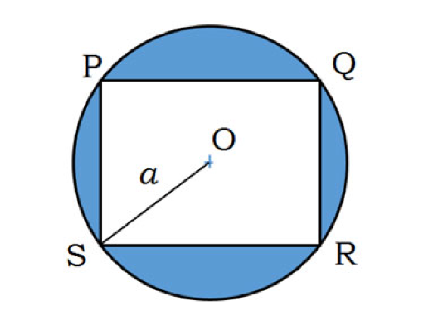
\includegraphics[width=0.3\textwidth]{figs/fig1.png}
    \caption{}
    \label{fig:ga_q8}
\end{figure}
\begin{multicols}{2}
\begin{enumerate}
    \item $\pi a^{2}-a^{2}$
    \item $\pi a^{2}-\sqrt{2}a^{2}$
    \item $\pi a^{2}-2a^{2}$
    \item $\pi a^{2}-3a^{2}$
\end{enumerate}
\end{multicols}

\item a, b, c are real numbers. The quadratic equation $ax^{2}-bx+c=0$ has equal roots, which is $\beta$, then

\hfill{\brak{\text{GATE GG 2020}}}
\begin{multicols}{2}
\begin{enumerate}
    \item $\beta=b/a$
    \item $\beta^{2}=ac$
    \item $\beta^{3}=bc/(2a^{2})$
    \item $b^{2}\ne4ac$
\end{enumerate}
\end{multicols}

\item The following figure shows the data of students enrolled in 5 years (2014 to 2018) for two schools P and Q. During this period, the ratio of the average number of the students enrolled in school P to the average of the difference of the number of students enrolled in schools P and Q is

\hfill{\brak{\text{GATE GG 2020}}}
\begin{figure}[h!]
    \centering
    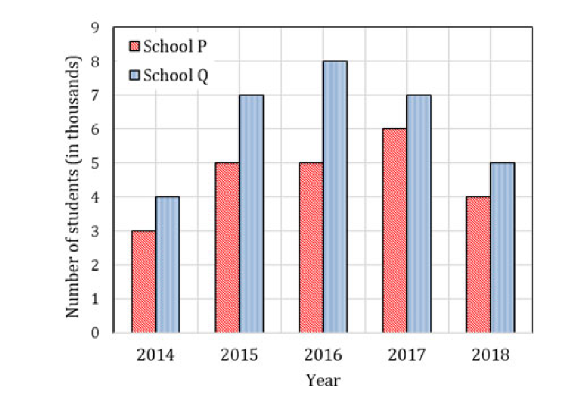
\includegraphics[width=0.7\textwidth]{figs/fig2.png}
    \caption{}
    \label{fig:ga_q10}
\end{figure}
\begin{multicols}{4}
\begin{enumerate}
    \item 8:23
    \item 23:8
    \item 23:31
    \item 31:23
\end{enumerate}
\end{multicols}



\newpage
\section*{Part A - Compulsory Section For All Candidates}



\item A plagioclase with $\frac{\text{Na}^{+}}{\text{Na}^{+}+\text{Ca}^{2+}}=0.8$ is

\hfill{\brak{\text{GATE GG 2020}}}
\begin{multicols}{4}
\begin{enumerate}
    \item albite
    \item anorthite
    \item oligoclase
    \item bytownite
\end{enumerate}
\end{multicols}

\item Tillite is an important constituent of the

\hfill{\brak{\text{GATE GG 2020}}}
\begin{multicols}{2}
\begin{enumerate}
    \item Talchir Formation
    \item Barakar Formation
    \item Pachmarhi Formation
    \item Lameta Formation
\end{enumerate}
\end{multicols}

\item If the ratio of gravity to total magnetic field at the equator of the Earth is X, then the ratio of gravity to total magnetic field at the pole of the Earth will be close to

\hfill{\brak{\text{GATE GG 2020}}}
\begin{multicols}{4}
\begin{enumerate}
    \item 2X
    \item X/2
    \item 4X
    \item X/8
\end{enumerate}
\end{multicols}

\item Which of the following is NOT a point group?

\hfill{\brak{\text{GATE GG 2020}}}
\begin{multicols}{4}
\begin{enumerate}
    \item 222
    \item 422
    \item 432
    \item 632
\end{enumerate}
\end{multicols}

\item Mississippian is an Epoch within the

\hfill{\brak{\text{GATE GG 2020}}}
\begin{multicols}{2}
\begin{enumerate}
    \item Permian Period
    \item Carboniferous Period
    \item Triassic Period
    \item Jurassic Period
\end{enumerate}
\end{multicols}

\item The given stereoplot of the axial plane and the axis of a fold represents an/a

\hfill{\brak{\text{GATE GG 2020}}}
\begin{figure}[h!]
    \centering
    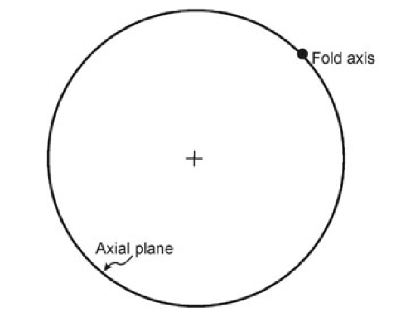
\includegraphics[width=0.3\textwidth]{figs/fig3.png}
    \caption{}
    \label{fig:partA_q6}
\end{figure}
\begin{multicols}{2}
\begin{enumerate}
    \item upright fold
    \item vertical fold
    \item reclined fold
    \item recumbent fold
\end{enumerate}
\end{multicols}

\item A siliciclastic sedimentary rock with $<$5\% matrix and QFL composition of 60\% quartz, 30\% rock fragments and 10\% feldspar, is called

\hfill{\brak{\text{GATE GG 2020}}}
\begin{multicols}{2}
\begin{enumerate}
    \item quartz wacke
    \item lithic arenite
    \item quartz arenite
    \item feldspathic wacke
\end{enumerate}
\end{multicols}

\item Which one of the following pairs of geophysical methods is most suitable to delineate chromite ore deposits occurring at a shallow depth in a granitic terrain?

\hfill{\brak{\text{GATE GG 2020}}}
\begin{multicols}{2}
\begin{enumerate}
    \item Gravity and Electrical methods
    \item Electrical and Electromagnetic methods
    \item Seismic and Gravity methods
    \item Seismic and Magnetic methods
\end{enumerate}
\end{multicols}

\item The ratio of bridging to non-bridging oxygen atoms is zero in case of

\hfill{\brak{\text{GATE GG 2020}}}
\begin{multicols}{2}
\begin{enumerate}
    \item nesosilicates
    \item inosilicates
    \item phyllosilicates
    \item tectosilicates
\end{enumerate}
\end{multicols}

\item Lahar is a geomorphic feature associated with

\hfill{\brak{\text{GATE GG 2020}}}
\begin{multicols}{2}
\begin{enumerate}
    \item wind activity
    \item river activity
    \item glacial activity
    \item volcanic activity
\end{enumerate}
\end{multicols}

\item Kepler's second law of planetary motion follows the principle of conservation of

\hfill{\brak{\text{GATE GG 2020}}}
\begin{multicols}{2}
\begin{enumerate}
    \item energy
    \item momentum
    \item angular momentum
    \item moment of inertia
\end{enumerate}
\end{multicols}

\item Which one of the following options shows the internal structural units of the Earth arranged in the CORRECT sequence of increasing volume?

\hfill{\brak{\text{GATE GG 2020}}}
\begin{enumerate}
    \item Outer core $<$ Inner core $<$ Upper mantle $<$ Lower mantle
    \item Outer core $<$ Inner core $<$ Lower mantle $<$ Upper mantle
    \item Inner core $<$ Outer core $<$ Upper mantle $<$ Lower mantle
    \item Inner core $<$ Outer core $<$ Lower mantle $<$ Upper mantle
\end{enumerate}

\item Which one of the following is NOT an earthquake intensity scale?

\hfill{\brak{\text{GATE GG 2020}}}
\begin{multicols}{2}
\begin{enumerate}
    \item Richter scale
    \item JMA scale
    \item Modified Mercalli scale
    \item Rossi-Forel scale
\end{enumerate}
\end{multicols}

\item The dimension of transmissivity of an aquifer is

\hfill{\brak{\text{GATE GG 2020}}}
\begin{multicols}{2}
\begin{enumerate}
    \item $M^{0}L^{1}T^{-1}$
    \item $M^{0}L^{0}T^{0}$
    \item $M^{1}L^{-1}T^{-2}$
    \item $M^{0}L^{2}T^{-1}$
\end{enumerate}
\end{multicols}




\item During 'K-capture' nuclear transmutation process

\hfill{\brak{\text{GATE GG 2020}}}
\begin{enumerate}
    \item both atomic number and atomic mass increase
    \item atomic number decreases but atomic mass remains the same
    \item atomic number increases but atomic mass remains the same
    \item both atomic number and atomic mass decrease
\end{enumerate}

\item Which one amongst the following logs has the maximum depth of investigation?

\hfill{\brak{\text{GATE GG 2020}}}
\begin{multicols}{2}
\begin{enumerate}
    \item Neutron log
    \item Natural Gamma-ray log
    \item Lateral log
    \item Density log
\end{enumerate}
\end{multicols}

\item The scale factor of an aerial photo of a planar ground surface, taken vertically downwards by a camera with a focal length of 300 mm, from a flying height of 3000 m is \rule{1cm}{0.15mm}.

\hfill{\brak{\text{GATE GG 2020}}}

\item In a soil sample, specific gravity of soil particles is 2.5 and the void ratio is 0.5. The density of the soil sample when it is fully saturated with water is \rule{1cm}{0.15mm} $kg/m^{3}$. (Assume density of water $=1000~kg/m^{3},$ and no volume change of the soil sample with saturation)

\hfill{\brak{\text{GATE GG 2020}}}

\item Nuclide A decays to nuclide B exclusively through $\alpha$ and $\beta$ decay, such that the mass number is reduced by 32 and the atomic number is reduced by 10. The number of $\beta$ particles emitted during the decay of nuclide A to nuclide B is \rule{1cm}{0.15mm}.

\hfill{\brak{\text{GATE GG 2020}}}

\item A cylindrical specimen (diameter $=54.7$ mm; length $=110$ mm) of basalt shows linear elastic behavior under uniaxial compression. At an axial stress of 100 Mega-Pascal (MPa), the absolute value of the measured axial strain is 0.2\%. The Young's modulus is calculated to be \rule{1cm}{0.15mm} Giga-Pascal (GPa).

\hfill{\brak{\text{GATE GG 2020}}}

\item A Mid-Oceanic-Ridge has symmetric magnetic anomalies about the ridge axis as shown below. Using the information given in the figure, the average relative velocity between the Plates A and B is calculated to be \rule{1cm}{0.15mm} cm/year.

\hfill{\brak{\text{GATE GG 2020}}}
\begin{figure}[h!]
    \centering
    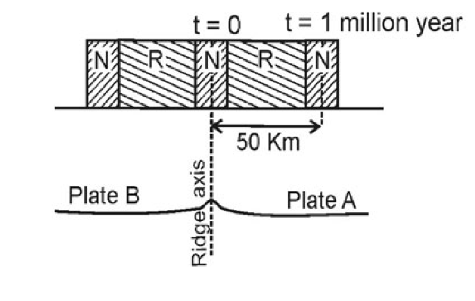
\includegraphics[width=0.7\textwidth]{figs/fig4.png}
    \caption{}
    \label{fig:partA_q21}
\end{figure}

\item The transmission coefficient for the vertically incident seismic wave at the interface between Layer 1 and Layer 2 given in the figure is \rule{1cm}{0.15mm}. (Round off to 2 decimal places)

\hfill{\brak{\text{GATE GG 2020}}}
\begin{figure}[h!]
    \centering
    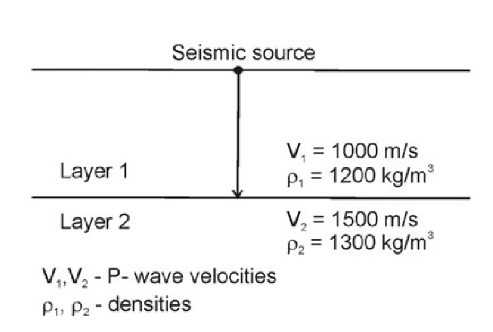
\includegraphics[width=0.5\textwidth]{figs/fig5.png}
    \caption{}
    \label{fig:partA_q22}
\end{figure}
\newpage
\item The geometrical factor for the electrode configuration given below will be \rule{1cm}{0.15mm} m. (Round off to 2 decimal places) (Use $\pi=3.14$) \\ ($C_{1}$ and $C_{2}$ are current electrodes; $P_{1}$ and $P_{2}$ are potential electrodes)

\hfill{\brak{\text{GATE GG 2020}}}
\begin{figure}[h!]
    \centering
    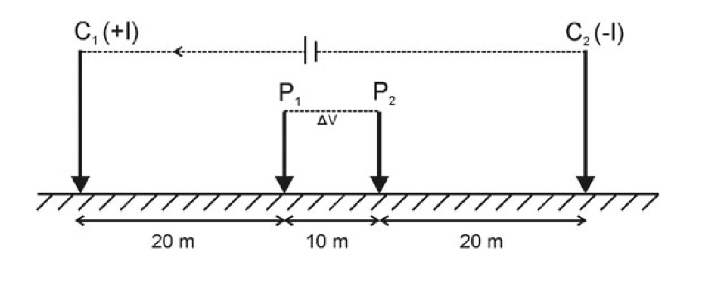
\includegraphics[width=0.8\textwidth]{figs/fig6.png}
    \caption{}
    \label{fig:partA_q23}
\end{figure}

\item In an electromagnetic measurement, the resultant field shows a phase lag of $30^{\degree}$ with respect to the primary field at the receiver coil. The ratio of Inphase to Quadrature component of the resultant field is \rule{1cm}{0.15mm}. (Round off to 2 decimal places)

\hfill{\brak{\text{GATE GG 2020}}}

\item A 4 km-high plateau is isostatically compensated as shown in the figure. Assuming Pratt's hypothesis of isostasy, the calculated density of the plateau is \rule{1cm}{0.15mm} $kg/m^{3}$.

\hfill{\brak{\text{GATE GG 2020}}}
\begin{figure}[h!]
    \centering
    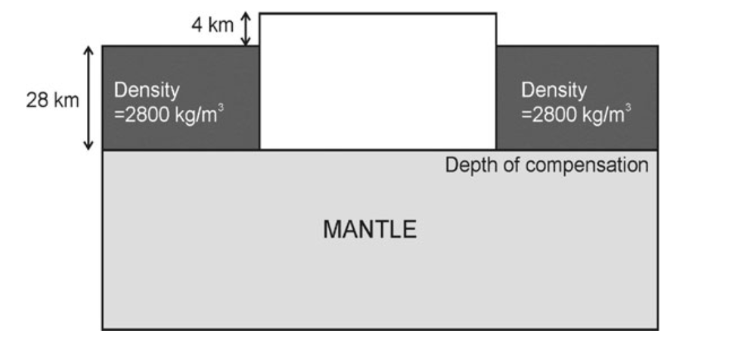
\includegraphics[width=0.7\textwidth]{figs/fig7.png}
    \caption{}
    \label{fig:partA_q25}
\end{figure}



\newpage
\section*{Part B (Section 1): For Geology Candidates Only}



\item ``Point Group'' in crystallography is characterized by a set of symmetry operations such that

\hfill{\brak{\text{GATE GG 2020}}}
\begin{enumerate}
    \item all points in a crystal are affected by it
    \item no point in a crystal is affected by it
    \item at least one point in a crystal is affected by it
    \item at least one point in a crystal is unaffected by it
\end{enumerate}

\item What are the Miller indices of a plane that intercepts each of the crystallographic axes X, Y and Z, at 2 \AA? (Assume a primitive unit-cell with the dimensions $a=5$ \AA, $b=2$ \AA~ and $c=4$ \AA.)

\hfill{\brak{\text{GATE GG 2020}}}
\begin{multicols}{4}
\begin{enumerate}
    \item (111)
    \item (524)
    \item (425)
    \item (542)
\end{enumerate}
\end{multicols}

\item Which one of the following processes is associated with the emission of X-rays?

\hfill{\brak{\text{GATE GG 2020}}}
\begin{multicols}{2}
\begin{enumerate}
    \item alpha decay
    \item beta decay
    \item electron capture decay
    \item positron decay
\end{enumerate}
\end{multicols}

\item Which one of the following radioisotopes has the longest half-life?

\hfill{\brak{\text{GATE GG 2020}}}
\begin{multicols}{4}
\begin{enumerate}
    \item $^{87}Rb$
    \item $^{147}Sm$
    \item $^{232}Th$
    \item $^{238}U$
\end{enumerate}
\end{multicols}

\item The given geological map represents

\hfill{\brak{\text{GATE GG 2020}}}
\begin{figure}[h!]
    \centering
    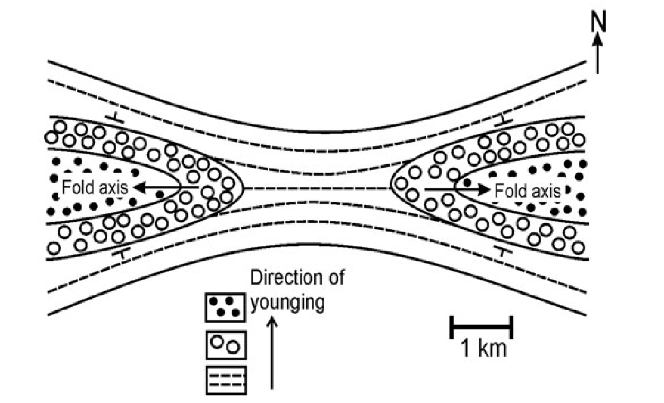
\includegraphics[width=0.8\textwidth]{figs/fig8.png}
    \caption{}
    \label{fig:partB_geo_q5}
\end{figure}
\begin{enumerate}
    \item culmination of an antiformal anticline
    \item culmination of an antiformal syncline
    \item depression of a synformal anticline
    \item culmination of a synformal syncline
\end{enumerate}

\item On a fault plane, the net slip is parallel to the bedding trace. Then, the apparent movement will be recognizable

\hfill{\brak{\text{GATE GG 2020}}}
\begin{enumerate}
    \item both in horizontal and vertical sections
    \item in horizontal, but not in vertical section
    \item in vertical, but not in horizontal section
    \item neither in horizontal nor in vertical section
\end{enumerate}

\item The CORRECT sequence of the given electromagnetic radiations in order of increasing wavelength is

\hfill{\brak{\text{GATE GG 2020}}}
\begin{enumerate}
    \item Ultraviolet $<$ Gamma Rays $<$ Radiowave $<$ Near-Infrared
    \item Gamma Rays $<$ Ultraviolet $<$ Near-Infrared $<$ Radiowave
    \item Gamma Rays $<$ Radiowave $<$ Ultraviolet $<$ Near-Infrared
    \item Ultraviolet $<$ Radiowave $<$ Near-Infrared $<$ Gamma Rays
\end{enumerate}

\item Choose the CORRECT combination of foraminiferal tests and types of coiling.

\hfill{\brak{\text{GATE GG 2020}}}
\begin{figure}[h!]
    \centering
    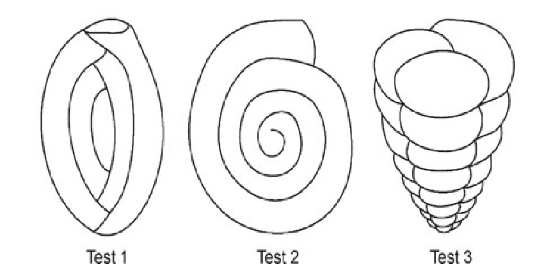
\includegraphics[width=0.9\textwidth]{figs/fig9.png}
    \caption{}
    \label{fig:partB_geo_q8}
\end{figure}
\begin{enumerate}
    \item Test 1-Trochospiral, Test 2 - Planispiral, Test 3 - Milioline
    \item Test 1-Milioline, Test 2- Planispiral, Test 3- Trochospiral
    \item Test 1- Milioline, Test 2 - Trochospiral, Test 3- Planispiral
    \item Test 1- Trochospiral, Test 2- Milioline, Test 3- Planispiral
\end{enumerate}

\item The figure below represents an isobaric binary liquidus phase diagram, with the solid phases A, B and C. What are the degrees of freedom associated with equilibrium phase assemblages represented by the bulk compositions w, x, y and z, in the fields indicated in the figure?

\hfill{\brak{\text{GATE GG 2020}}}
\begin{figure}[h!]
    \centering
    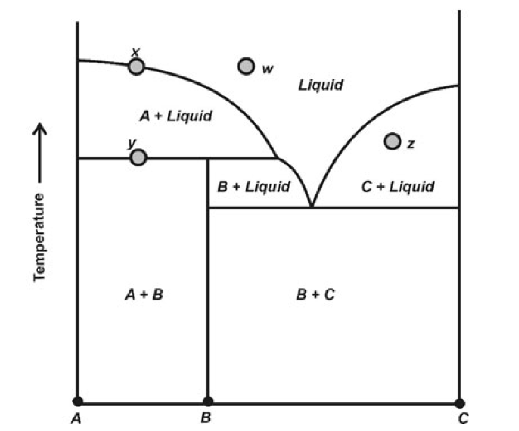
\includegraphics[width=0.7\textwidth]{figs/fig10.png}
    \caption{}
    \label{fig:partB_geo_q9}
\end{figure}
\begin{multicols}{2}
\begin{enumerate}
    \item $w=2, x=1, y=1, z=1$
    \item $w=2, x=1, y=0, z=2$
    \item $w=1, x=1, y=0, z=1$
    \item $w=1, x=1, y=1, z=2$
\end{enumerate}
\end{multicols}

\item Match the basins (Group I) with the corresponding stratigraphic units (Group II).

\hfill{\brak{\text{GATE GG 2020}}}

\begin{tabular}{ll|ll}
\multicolumn{2}{c}{\textbf{Group I}} & \multicolumn{2}{c}{\textbf{Group II}} \\

1. & Kerur Formation & P. & Cuddapah \\
2. & Dhandraul Quartzite & Q. & Chattisgarh \\
3. & Bairenkonda Quartzite & R. & Kaladgi-Badami \\
4. & Gunderdehi Formation & S. & Vindhyan \\
\end{tabular}

\begin{multicols}{2}
\begin{enumerate}
    \item P-3, Q-4, R-1, S-2
    \item P-2, Q-4, R-1, S-3
    \item P-3, Q-1, R-4, S-2
    \item P-2, Q-3, R-4, S-1
\end{enumerate}
\end{multicols}

\item In the metamorphic reaction \\ Quartz + Muscovite = X + Sillimanite + Water, `X' represents

\hfill{\brak{\text{GATE GG 2020}}}
\begin{multicols}{2}
\begin{enumerate}
    \item Garnet
    \item Staurolite
    \item Orthoclase
    \item Cordierite
\end{enumerate}
\end{multicols}

\item The talc-kyanite assemblage can stabilize in

\hfill{\brak{\text{GATE GG 2020}}}
\begin{multicols}{2}
\begin{enumerate}
    \item greenschist facies marly rocks
    \item amphibolite facies mafic rocks
    \item eclogite facies pelitic rocks
    \item sanidinite facies ultramafic rocks
\end{enumerate}
\end{multicols}

\item Which one of the following statements about igneous rocks is CORRECT?

\hfill{\brak{\text{GATE GG 2020}}}
\begin{enumerate}
    \item Tholeiitic and calc-alkaline rocks are both alkaline in nature.
    \item Tholeiitic rocks are subalkaline, but calc-alkaline rocks are alkaline in nature.
    \item Tholeiitic rocks are alkaline, but calc-alkaline rocks are subalkaline in nature.
    \item Tholeiitic and calc-alkaline rocks are both subalkaline in nature.
\end{enumerate}

\item Based on the three statements given below, choose the CORRECT option.\\
Statement I: Barchans are crescent-shaped dunes that close in the downwind direction.\\
Statement II: Parabolic dunes are U-shaped dunes that close in the downwind direction.\\
Statement III: Barchanoid dunes are sinuous transverse ridges, the crestline sinuosity of successive bedforms are either in-phase or out-phase.

\hfill{\brak{\text{GATE GG 2020}}}
\begin{enumerate}
    \item All the statements are correct
    \item Statement I is correct, but statements II and III are incorrect
    \item Statements I and II are correct, but statement III is incorrect
    \item Statements II and III are correct, but statement I is incorrect
\end{enumerate}

\item Based on the three statements given below, choose the CORRECT option.\\
Statement I: Barapasaurus is known from the Jurassic Kota Formation.\\
Statement II: Morganucodon is known from the Tatrot Formation.\\
Statement III: Lystrosaurus is known from the Lameta Formation.

\hfill{\brak{\text{GATE GG 2020}}}
\begin{enumerate}
    \item All the three statements are correct
    \item Statement I is correct but statements II and III are incorrect
    \item Statements I and II are correct but statement III is incorrect
    \item Statements II and III are correct but statement I is incorrect
\end{enumerate}

\item Which one of the following assemblages of plant fossils is known from the Barakar Formation?

\hfill{\brak{\text{GATE GG 2020}}}
\begin{multicols}{2}
\begin{enumerate}
    \item Glossopteris, Gangamopteris, Dicroidium
    \item Glossopteris, Gangamopteris, Noeggerathiopsis
    \item Glossopteris, Gangamopteris, Ptilophyllum
    \item Schizoneura, Noeggerathiopsis, Ptilophyllum
\end{enumerate}
\end{multicols}

\item Match the features (Group I) with the corresponding invertebrate genera (Group II).

\hfill{\brak{\text{GATE GG 2020}}}

\begin{tabular}{ll|ll}
\multicolumn{2}{c}{\textbf{Group I}} & \multicolumn{2}{c}{\textbf{Group II}} \\
\hline
P. & Cardinal Fossula & 1. & Calymene \\
Q. & Chrondrophore & 2. & Rhynchonella \\
R. & Lophophore & 3. & Zaphrentis \\
S. & Glabella & 4. & Mya \\
\end{tabular}

\begin{multicols}{2}
\begin{enumerate}
    \item P-3, Q-4, R-1, S-2
    \item P-3, Q-4, R-2, S-1
    \item P-4, Q-3, R-2, S-1
    \item P-2, Q-1, R-4, S-3
\end{enumerate}
\end{multicols}

\item If the orthogonal thickness is constant along a folded layer, as per Ramsay's morphological classification of folds, it is a

\hfill{\brak{\text{GATE GG 2020}}}
\begin{multicols}{4}
\begin{enumerate}
    \item Class 1A fold
    \item Class 1B fold
    \item Class 1C fold
    \item Class 2 fold
\end{enumerate}
\end{multicols}

\item If density of quartz is 2650 kg/m$^3$ and that of orthoclase is 2550 kg/m$^3$, the lithostatic pressure due to a granite with 68 modal \% quartz and 32 modal \% orthoclase at a depth of 10 km will be \rule{1cm}{0.15mm} kbar. (Round off to 2 decimal places) (Acceleration due to gravity, g=9.8 m/s$^2$)

\hfill{\brak{\text{GATE GG 2020}}}

\item The unit-cell of an orthorhombic mineral was compressed during deformation from 5 \AA~ to 4.5 \AA~ along the c-axis, with the other two dimensions remaining unaffected. The absolute value of the shift in the position of the (001) peak in its XRD pattern is \rule{1cm}{0.15mm} $^{\degree}2\theta$. (Round off to 3 decimal places) (Wavelength of X-ray used = 1.5418 \AA. For orthorhombic system: $1/d^2 = h^2/a^2 + k^2/b^2 + l^2/c^2$)

\hfill{\brak{\text{GATE GG 2020}}}

\item The grade of iron in an ore body containing 80 wt. \% hematite and 20 wt. \% gangue is \rule{1cm}{0.15mm} \%. (Round off to 2 decimal places) (Atomic wt. of Fe = 55.85; atomic weight of O = 16).

\hfill{\brak{\text{GATE GG 2020}}}

\item The abundances of the isotopes $^{35}$Cl (atomic mass = 34.96885 amu) and $^{37}$Cl (atomic mass = 36.96590 amu) are 75.77 \% and 24.23 \%, respectively. The calculated atomic weight of Cl is \rule{1cm}{0.15mm} amu. (Round off to 3 decimal places)

\hfill{\brak{\text{GATE GG 2020}}}

\item A vertical profile perpendicular to the crest line of an asymmetrical ripple is given in the figure. The calculated Ripple Index is \rule{1cm}{0.15mm}.

\hfill{\brak{\text{GATE GG 2020}}}
\begin{figure}[h!]
    \centering
    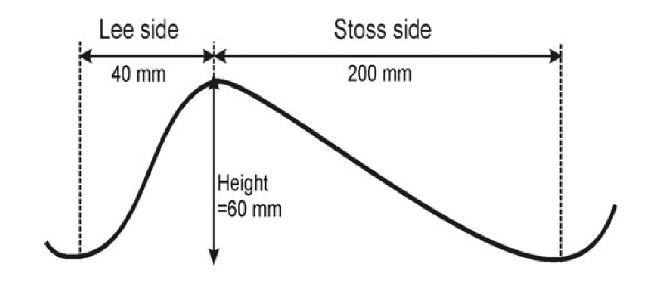
\includegraphics[width=0.7\textwidth]{figs/fig11.png}
    \caption{}
    \label{fig:partB_geo_q23}
\end{figure}

\item A source rock undergoes melting. Assuming batch melting, 5\% partial melting and bulk distribution coefficient of 0.045, the enrichment factor (C$_L$/C$_0$) of Rb in the melt will be \rule{1cm}{0.15mm}. (Round off to 2 decimal places)

\hfill{\brak{\text{GATE GG 2020}}}

\item If the $\Delta$H of formation of CaSiO$_3$, SiO$_2$ and CaO from Ca, Si and O are respectively -1635, -911 and -635 kJ/mol, the enthalpy of formation of CaSiO$_3$ from CaO and SiO$_2$ is \rule{1cm}{0.15mm} kJ/mol.

\hfill{\brak{\text{GATE GG 2020}}}

\item The tip-line of an actively propagating thrust fault is located at a depth of 1 km from the horizontal ground surface. The average density of the material from the ground surface to this depth is assumed to be uniform and can be taken as 2700 kg/m$^3$. The rock at this depth follows the failure criterion given by the equation $\sigma_1 = 10 \text{MPa} + 3\sigma_3$, where $\sigma_1$ and $\sigma_3$ are the maximum and minimum principal stresses. Considering Anderson's theory of faulting, the calculated maximum principal stress at this depth is \rule{1cm}{0.15mm} Mega-Pascal (MPa). (Assume the acceleration due to gravity (g) to be 10 m/s$^2$)

\hfill{\brak{\text{GATE GG 2020}}}

\item During a rockslide, a 20 kg granite block gets dislodged from the top of a planar hill slope and starts sliding down the slope as shown in the figure. The slope angle is 30$^{\degree}$ with the horizontal. After travelling a distance of 40 m in the same direction on the slope, the block hits the road. Assuming zero cohesion and zero friction and considering acceleration due to gravity (g) as 10 m/s$^2$, the velocity with which the block hits the road is \rule{1cm}{0.15mm} m/s.

\hfill{\brak{\text{GATE GG 2020}}}
\begin{figure}[h!]
    \centering
    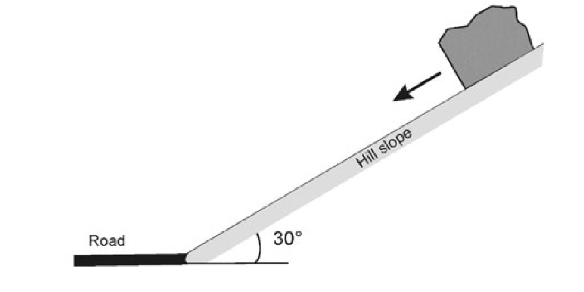
\includegraphics[width=0.7\textwidth]{figs/fig12.png}
    \caption{}
    \label{fig:partB_geo_q27}
\end{figure}

\item Liquid limit and plastic limit of a soil are 40\% and 20\%, respectively. If the natural (i.e. \textit{in situ}) water content of the soil is 30\%, the liquidity index is \rule{1cm}{0.15mm}.

\hfill{\brak{\text{GATE GG 2020}}}

\item A confined aquifer has a uniform area (`A') perpendicular to the water flow. The hydraulic gradient and coefficient of permeability are given as 0.005 and 2 m/day, respectively. The total daily flow of water is 250 m$^3$. Using Darcy's law, the calculated value of `A' is \rule{1cm}{0.15mm} m$^2$.

\hfill{\brak{\text{GATE GG 2020}}}

\item The apparent dip amount of a sandstone bed is 45$^{\degree}$. The angle between the true dip direction and the apparent dip direction is 60$^{\degree}$. The true dip amount of the bed is \rule{1cm}{0.15mm} degree ($^{\degree}$). (Round off to 2 decimal places)

\hfill{\brak{\text{GATE GG 2020}}}









\section*{PART B (Section 2): For Geophysics Candidates Only}



\item International gravity formula is based on which one of the following models?

\hfill{\brak{\text{GATE GG 2020}}}
\begin{enumerate}
    \item Non-rotating homogeneous spherical Earth model
    \item Non-rotating homogeneous oblate spheroidal Earth model
    \item Rotating homogeneous oblate spheroidal Earth model
    \item Rotating inhomogeneous spherical Earth model
\end{enumerate}

\item Heat flow equation $\frac{d^2T}{dz^2} = 0$ is valid when \\


\hfill{\brak{\text{GATE GG 2020}}}
\begin{enumerate}
    \item steady state heat conduction is considered in an isotropic medium without heat source
    \item steady state heat conduction is considered in an isotropic medium with heat source
    \item steady state heat convection is considered in an isotropic medium without heat source
    \item steady state heat convection is considered in an isotropic medium with heat source
\end{enumerate}

\item Assuming the inner core of the Earth to be one-third of its present size, which one of the following statements is CORRECT? (Radius of the Earth and outer core remain unchanged)

\hfill{\brak{\text{GATE GG 2020}}}
\begin{enumerate}
    \item Shadow zones of both P-wave and S-wave increase
    \item Shadow zone of P-wave increases and that of S-wave remains unchanged
    \item Shadow zones of both P-wave and S-wave decrease
    \item Shadow zone of P-wave decreases but that of S-wave remains unchanged
\end{enumerate}

\item Match the following instruments (Group I) with their corresponding physical principle (Group II).

\hfill{\brak{\text{GATE GG 2020}}}
\begin{center}
\begin{tabular}{ll|ll}
\multicolumn{2}{c}{\textbf{Group I}} & \multicolumn{2}{c}{\textbf{Group II}} \\
\hline
P. & Fluxgate magnetometer & 1. & Hooke's law \\
Q. & LaCoste-Romberg gravimeter & 2. & Zeeman effect \\
R. & Proton Precession magnetometer & 3. & Faraday's law of EM-induction \\
S. & Optically pumped magnetometer & 4. & Nuclear magnetic resonance \\
\end{tabular}
\end{center}
\begin{multicols}{2}
\begin{enumerate}
    \item P-1, Q-2, R-4, S-3
    \item P-4, Q-3, R-2, S-1
    \item P-3, Q-1, R-4, S-2
    \item P-3, Q-2, R-4, S-1
\end{enumerate}
\end{multicols}

\item The sensitivity of LaCoste-Romberg gravimeter is proportional to the time period (T) of the spring as

\hfill{\brak{\text{GATE GG 2020}}}
\begin{multicols}{4}
\begin{enumerate}
    \item $T^2$
    \item $1/T^2$
    \item $\sqrt{T}$
    \item $1/\sqrt{T}$
\end{enumerate}
\end{multicols}

\item Match the following gravity/magnetic data interpretation techniques (Group I) with the corresponding terms (Group II).

\hfill{\brak{\text{GATE GG 2020}}}
\begin{center}
\begin{tabular}{ll|ll}
\multicolumn{2}{c}{\textbf{Group I}} & \multicolumn{2}{c}{\textbf{Group II}} \\
\hline
P. & Euler deconvolution & 1. & Symmetry \\
Q. & Power spectrum analysis & 2. & Source response enhancement \\
R. & Reduced to pole transformation & 3. & Equation of homogeneity \\
S. & Downward continuation & 4. & Basement depth \\
\end{tabular}
\end{center}
\begin{multicols}{2}
\begin{enumerate}
    \item P-1, Q-2, R-4, S-3
    \item P-3, Q-4, R-1, S-2
    \item P-1, Q-2, R-1, S-3
    \item P-3, Q-1, R-4, S-2
\end{enumerate}
\end{multicols}

\item Assuming uncorrelated noise, the improvement in the signal to noise ratio in a reflection seismic survey with `n' geophones spaced equally along the profile is proportional to

\hfill{\brak{\text{GATE GG 2020}}}
\begin{multicols}{4}
\begin{enumerate}
    \item $n$
    \item $1/n$
    \item $\sqrt{n}$
    \item $1/\sqrt{n}$
\end{enumerate}
\end{multicols}



\item A waveform with amplitude spectrum A($\omega$) and phase spectrum $\phi(\omega)$ is auto-correlated. Which one of the options given below correctly represents the information about the original waveform that can be retrieved from the auto-correlated waveform?

\hfill{\brak{\text{GATE GG 2020}}}
\begin{enumerate}
    \item A($\omega$) can be retrieved but not $\phi(\omega)$
    \item $\phi(\omega)$ can be retrieved but not A($\omega$)
    \item Both A($\omega$) and $\phi(\omega)$ can be retrieved
    \item Both A($\omega$) and $\phi(\omega)$ cannot be retrieved
\end{enumerate}

\item The convolution of A = \{4, -2, -1, 2\} with B = \{1, 0, -1\} gives

\hfill{\brak{\text{GATE GG 2020}}}
\begin{multicols}{2}
\begin{enumerate}
    \item \{4, -2, -5, 4, 1, -2\}
    \item \{4, 2, -5, 0, 1, -2\}
    \item \{4, -2, -5, 0, -1, -2\}
    \item \{4, -2, 0, 4, 1, -2\}
\end{enumerate}
\end{multicols}

\item Which one of the following does NOT contribute to the suppression of SP log response for a thin, shaly, gas-bearing sandstone formation? (Resistivity of mud filtrate $>$ resistivity of formation water)

\hfill{\brak{\text{GATE GG 2020}}}
\begin{enumerate}
    \item Increase in shale content
    \item Increase in hydrocarbon content
    \item Decrease in bed thickness
    \item Increase in the salinity of formation water
\end{enumerate}

\item The crossover observed for a hydrocarbon-bearing sandstone formation in the plot of Neutron and Density porosity logs ($\phi_n$ = Neutron porosity and $\phi_d$ = Density porosity) is due to

\hfill{\brak{\text{GATE GG 2020}}}
\begin{enumerate}
    \item increase in $\phi_d$ and decrease in $\phi_n$
    \item decrease in $\phi_d$ and increase in $\phi_n$
    \item increase in both $\phi_d$ and $\phi_n$
    \item decrease in both $\phi_d$ and $\phi_n$
\end{enumerate}

\item In which one of the following electromagnetic methods are the amplitude ratio and relative phase difference measured between two receiver coils?

\hfill{\brak{\text{GATE GG 2020}}}
\begin{multicols}{2}
\begin{enumerate}
    \item Fixed vertical loop method
    \item Compensator method
    \item TURAM method
    \item Slingram method
\end{enumerate}
\end{multicols}

\item If four impedance tensors $Z_{xx}, Z_{yy}, Z_{xy}$ and $Z_{yx}$ are computed for a 2D body in magneto-telluric method (x is the strike direction), then

\hfill{\brak{\text{GATE GG 2020}}}
\begin{enumerate}
    \item $Z_{xx} = 0, Z_{yy} \ne 0, Z_{xy} = Z_{yx}$
    \item $Z_{xx} \ne 0, Z_{yy} = 0, Z_{xy} = Z_{yx}$
    \item $Z_{xx} \ne 0, Z_{yy} \ne 0, Z_{xy} \ne Z_{yx}$
    \item $Z_{xx} = 0, Z_{yy} = 0, Z_{xy} \ne Z_{yx}$
\end{enumerate}

\item Match the inversion methods (Group I) with the associated terms (Group II).

\hfill{\brak{\text{GATE GG 2020}}}
\begin{center}
\begin{tabular}{ll|ll}
\multicolumn{2}{c}{\textbf{Group I}} & \multicolumn{2}{c}{\textbf{Group II}} \\
\hline
P. & Genetic algorithm & 1. & Lagrange multiplier \\
Q. & Simulated annealing & 2. & Fitness \\
R. & Least squares inverse & 3. & Energy \\
S. & Minimum norm least squares inverse & 4. & Damping \\
\end{tabular}
\end{center}
\begin{multicols}{2}
\begin{enumerate}
    \item P-3, Q-2, R-1, S-4
    \item P-4, Q-3, R-1, S-2
    \item P-2, Q-1, R-4, S-3
    \item P-2, Q-3, R-4, S-1
\end{enumerate}
\end{multicols}




\item Ten equispaced metal electrodes are arranged along a profile for multi-electrode 2D resistivity imaging survey. If Wenner array is used for data recording, the maximum number of observations will be

\hfill{\brak{\text{GATE GG 2020}}}
\begin{multicols}{4}
\begin{enumerate}
    \item 7
    \item 11
    \item 13
    \item 15
\end{enumerate}
\end{multicols}

\item P and R are Jacobian matrices for two different geophysical inverse problems. If their generalized inverses are written as $P^{-g} = (P^T P)^{-1} P^T$ and $R^{-g} = R^T(R R^T)^{-1}$, then

\hfill{\brak{\text{GATE GG 2020}}}
\begin{enumerate}
    \item P represents an overdetermined problem and R represents an underdetermined problem
    \item P represents an underdetermined problem and R represents an overdetermined problem
    \item Both P and R represent overdetermined problems
    \item Both P and R represent underdetermined problems
\end{enumerate}


\item In a 3D seismic survey, there are 512 groups of receivers in one line of a patch. Eight groups are moved per line from one patch to the next along the swath. What is the inline fold?

\hfill{\brak{\text{GATE GG 2020}}}

\begin{multicols}{4}
\begin{enumerate}
\item 32
\item 16
\item 8
\item 4
\end{enumerate}
\end{multicols}


\item The magnetic potential of a uniform vertically magnetized buried spherical body with uniform density is given as 
\[
W = \frac{\mu_0}{4\pi G} \frac{I}{\rho} g_z
\]
Then, the vertical magnetic field $B_z$ is proportional to

\hfill{\brak{\text{GATE GG 2020}}}

\begin{multicols}{2}
\begin{enumerate}
\item $\dfrac{2z^2-x^2}{(z^2+x^2)^{5/2}}$
\item $\dfrac{2z^2-x^2}{(z^2+x^2)^{3/2}}$
\item $\dfrac{z^2-x^2}{(z^2+x^2)^{5/2}}$
\item $\dfrac{z^2-x^2}{(z^2+x^2)^{3/2}}$
\end{enumerate}
\end{multicols}


\item A sample of granite is observed to have a P-wave velocity of $5 \, km/s$ and density of $2600 \, kg/m^3$. The bulk modulus of the granite, assuming it to be a Poisson’s solid, is \brak{\text{kPa}}. (Round off to 2 decimal places)

\hfill{\brak{\text{GATE GG 2020}}}


\item The half-life of a parent radionuclide is $100$ yrs. If the parent radionuclide decays to a daughter radionuclide which itself decays with a decay constant of $\tfrac{1}{4}$ that of the parent radionuclide, then radioactive equilibrium will be reached after \brak{\text{years}}. (Round off to 2 decimal places) (Assume at time $t=0$ the number of daughter radionuclide is zero)

\hfill{\brak{\text{GATE GG 2020}}}


\item Current and potential electrodes in resistivity survey over an inhomogeneous ground is shown in the figure below. If $100 \, mA$ current flow between $C_1$ and $C_2$ generates $50 \, mV$ potential difference between $P_1$ and $P_2$, then the apparent resistivity of the medium will be \brak{\text{$\Omega m$}}. (Round off to 2 decimal places) \\
\begin{figure}[h]
\centering
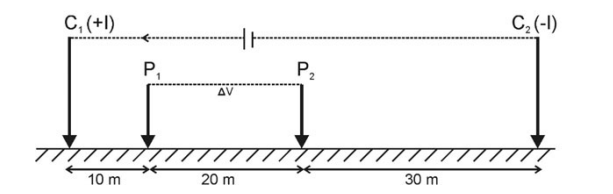
\includegraphics[width=0.5\textwidth]{figs/fig13.png}
\caption{}
\label{fig:q21}
\end{figure}

\hfill{\brak{\text{GATE GG 2020}}}


\item Skin depths in homogeneous media of resistivity $\rho_1$ and $\rho_2$ are $100 \, m$ and $200 \, m$, respectively, at $1000 \, Hz$ frequency. The ratio $\rho_1/\rho_2$ will be \brak{\text{}}. (Round off to 2 decimal places)

\hfill{\brak{\text{GATE GG 2020}}}


\item The mean resistivity of a horizontally stratified cuboid rock sample is $100 \, \Omega m$ and coefficient of electrical anisotropy is $1.15$. The transverse resistivity of the rock sample is \brak{\text{$\Omega m$}}. (Round off to 2 decimal places)

\hfill{\brak{\text{GATE GG 2020}}}


\item A seismic reflection survey is carried out over a $1500 \, m$ thick horizontal layer with a P-wave velocity of $2000 \, m/s$. The travel time of a reflected wave at a surface detector placed $1000 \, m$ from a surface source is \brak{\text{milliseconds}}.

\hfill{\brak{\text{GATE GG 2020}}}


\item A seismic reflection survey is carried out using a $10 \, ms$ seismic wavelet over a subsurface medium having an average P-wave velocity of $1600 \, m/s$. The best resolution obtained on the basis of Rayleigh criteria is \brak{\text{m}}. (Assume seismic wavelet contains one cycle)

\hfill{\brak{\text{GATE GG 2020}}}


\item To detect a $0.01 \, nT$ change in magnetic field using a proton precession magnetometer, the sensitivity required in the frequency measurement of the instrument is \brak{\text{$\times 10$ Hz}}. (Round off to 2 decimal places) (Assume gyromagnetic ratio of proton as $2.67515 \times 10^8 \, s^{-1}T^{-1}$)

\hfill{\brak{\text{GATE GG 2020}}}


\item A micro-gravity survey with appropriate station spacing is performed to detect a subsurface spherical cavity in a bedrock of density $2500 \, kg/m^3$. The depth to the center of the cavity is $4 \, m$ from the surface and the elevation measurement accuracy of the surveying instrument is $0.1 \, m$. The smallest cavity that can be detected by the survey must have a radius greater than \brak{\text{m}}. (Round off to 1 decimal place) (Assume $G = 6.673 \times 10^{-11} \, m^3kg^{-1}s^{-2}$)

\hfill{\brak{\text{GATE GG 2020}}}


\item The gravity anomaly over a spherical ore body is shown in the figure below. The calculated excess mass due to the ore body will be \brak{\text{$\times 10^{11} \, kg$}}. (Round off to 1 decimal place) \\
\begin{figure}[h]
\centering
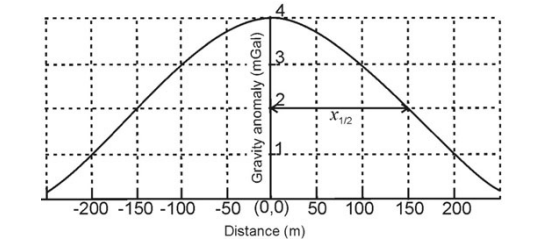
\includegraphics[width=0.5\textwidth]{figs/fig14.png}
\caption{}
\label{fig:q28}
\end{figure}

\hfill{\brak{\text{GATE GG 2020}}}


\item A scalar potential field in 3D space is expressed as 
\[
U(x,y,z) = x^2 + yz^2
\]
The magnitude of the maximum rate of change in $U(x,y,z)$ at a point $(1,1,2)$ is \brak{\text{}}.

\hfill{\brak{\text{GATE GG 2020}}}


\item A $10 \, Hz$ seismic wave propagates for $40 \, km$ through a material with a P-wave velocity of $5 \, km/s$ and quality factor $Q=100$. The percentage of the initial amplitude retained in the attenuated wave is \brak{\text{\%}}. (Round off to 1 decimal place) (Use $\pi = 3.14$)

\hfill{\brak{\text{GATE GG 2020}}}







\end{enumerate}

\begin{align*}
 {\LARGE{\textbf{END OF THE QUESTION PAPER}}}
\end{align*}



\end{document}